模板是C++的特性,这样函数和类可以支持泛型——可以实现独立于特定数据类型的函数或类,例如:客户端可以使用max()函数来处理不同的数据类型。不需要使用函数重载来实现和维护许多类似的函数,我们只需要实现一个max()并将数据类型作为参数传递。此外,模板可以与多重继承和操作符重载一起工作,从而在C++中可以创建强大的通用数据结构和算法,如:标准模板库(STL)。此外,模板还可以应用于编译时计算、编译时和运行时代码优化等。 \par
本章中,我们将学习函数和类模板的语法、它们的实例化和特化。然后,我们将介绍可变参数模板及其应用。接下来,将讨论模板参数和用于实例化它们的相应参数。之后,将学习如何实现一个类型特征,以及如何使用这种信息来优化算法。最后,将介绍一些可以用来提高程序执行速度的技术,包括编译时计算、编译时代码优化和静态多态性。\par
本章中,我们将了解以下内容: \par

\begin{itemize}
	\item 探索函数和类模板
	\item 了解可变模板
	\item 理解模板形参和参数
	\item 什么是特征?
	\item 模板元编程及其应用
\end{itemize}

\noindent\textbf{}\ \par
\textbf{源码位置} \ \par
本章的代码可以在这本书的GitHub中找到: https:/​/​github.com/​PacktPublishing/​Expert-​CPP . \par

\noindent\textbf{}\ \par
\textbf{探索函数和类模板} \ \par
我们将从介绍函数模板的语法开始,并通过实例化、推断类型和特化开始这一节。然后,转向类模板,看看类似的概念,以及示例。\par

\noindent\textbf{}\ \par
\textbf{动机} \ \par
目前为止,定义了函数或类时,必须提供输入、输出和中间参数。例如,有一个函数来执行两个int型整数的加法运算。如何扩展它,使它能够处理所有其他基本数据类型,如float、double、char等?一种方法是通过手动复制、粘贴和稍微修改每个函数来使用函数重载。另一种方法是定义一个宏来执行加法操作。这两种方法都有各自的副作用。 \par
此外,如果我们修复了一个bug或为一种类型添加了一个新特性,而这个更新需要对所有其他重载函数和类执行,这会导致什么情况?除了使用复制-粘贴-替换的方法,有更好的方法来处理这种情况吗? \par
事实上,这是任何计算机语言都可能面临的问题。这个问题由通用函数编程元语言(ML,Meta Language)在1973年提出,ML允许编写仅在使用时的类型集中使用不同的通用函数或类型,从而减少重复代码。后来,受Ada语言中生命保护(CLU,hartered life underwriter)提供的参数化模块和泛型的启发,C++采用了模板概念,它允许函数和类使用泛型类型进行操作。换句话说,它允许函数或类处理不同的数据类型,而不需要重新编写它们。 \par
实际上,从抽象的角度来看,C++函数或类模板可以作为创建其他类似函数或类的模式。这背后的基本思想是创建一个函数或类模板,而不必指定某些或所有变量的确切类型。我们使用占位符类型定义函数或类模板,称为模板类型形参。一旦有了函数或类模板,就可以使用在其他编译器中实现的算法自动生成函数或类。 \par
C++中有三种模板:函数模板、类模板和可变参数模板。接下来我们一个个的来了解。 \par

\noindent\textbf{}\ \par
\textbf{函数模板} \ \par
函数模板定义了如何生成一系列函数。这里是指一组行为相似的函数。如下图所示,这包括两个阶段: \par

\begin{itemize}
	\item 创建函数模板,书写的规则。
	\item 模板实例化,从模板中生成函数的规则:
\end{itemize}

\begin{center}
	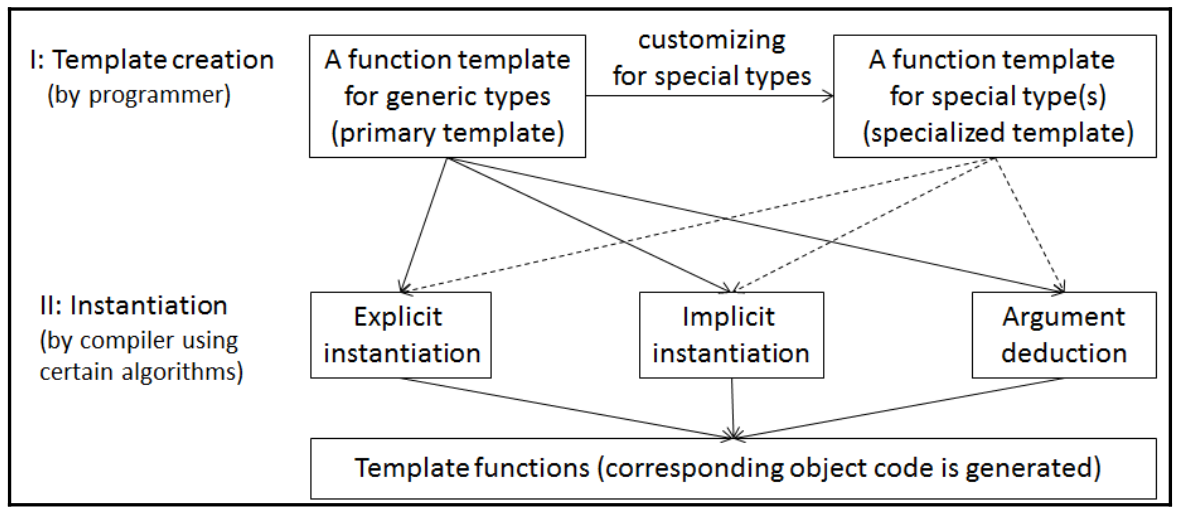
\includegraphics[width=0.6\textwidth]{content/Section-1/Chapter-4/1}
\end{center}

上图的\textbf{I}中,讨论了用于为泛型类型创建函数模板的格式,但与特化模板有关,我们也将特化模板称为主模板。\textbf{II }中,我们介绍从模板生成函数的三种方法。最后,特化和重载小节告诉我们如何为特殊类型定制主模板(通过改变其行为)。 \par

\noindent\textbf{}\ \par
\textbf{语法} \ \par
定义函数模板有两种方法,如下面的代码所示: \par

\begin{lstlisting}[caption={}]
template <typename identifier_1, …, typename identifier_n >
function_declaration;

template <class identifier_1,…, class identifier_n>
function_declaration;
\end{lstlisting}

这里,\texttt{identifier\underline{ }i (i=1,…,n)}是类型或类形参,而function\underline{ }declaration声明了部分函数体。前面两个声明的唯一区别是关键字——一个使用class,另一个使用typename,两者具有相同的含义和行为。因为类型(例如基本类型——int、float、double、enum、struct、union等)不是类,所以引入了typename关键字方法以避免混淆。 \par
例如,查找最大值函数模板app\underline{ }max()可以这样声明: \par

\begin{lstlisting}[caption={}]
template <class T>
T app_max (T a, T b) {
	return (a>b?a:b); //note: we use ((a)>(b) ? (a):(b)) in macros
}                     //it is safe to replace (a) by a, and (b) by b now
\end{lstlisting}

这个函数模板可以用于许多数据类型或类,只要有一个可复制构造的类型,其中表达式是a>b。对于用户定义的类,这意味着必须定义大于操作符(>)。 \par
注意,函数模板和模板函数是不同的东西。函数模板是一种编译器用来生成函数的模板,因此编译器不会为它生成任何目标代码。另一方面,模板函数是指函数模板中的一个实例。由于它是一个函数,相应的目标代码由编译器生成。然而,最新的C++标准文档建议避免使用不准确的术语定义模板函数。因此,本书将使用函数模板和成员函数模板。 \par

\noindent\textbf{}\ \par
\textbf{实例化} \ \par
因为可能有无限多个类型和类,函数模板的概念不仅节省了源代码的空间,而且使代码更容易阅读和维护。然而,与为应用程序中使用的不同数据类型编写单独的函数或类相比,模板不会产生更小的目标代码。例如,考虑一个使用float和int版本的app\underline{ }max()的程序: \par

\begin{lstlisting}[caption={}]
cout << app_max<int>(3,5) << endl;
cout << app_max<float>(3.0f,5.0f) << endl;
\end{lstlisting}

编译器将在目标文件中生成两个新函数,如下所示:\par

\begin{lstlisting}[caption={}]
int app_max<int> ( int a, int b) {
	return (a>b?a:b);
}

float app_max<float> (float a, float b) {
	return (a>b?a:b);
}
\end{lstlisting}

从函数模板声明创建函数的过程称为模板实例化。这个实例化过程中,编译器确定模板参数,并根据应用程序的需要生成实际的函数代码。实例化通常有三种形式:显式、隐式和推断。我们接下来讨论每一种形式。 \par

\noindent\textbf{}\ \par
\textbf{显式实例化} \ \par
很多非常有用的C++函数模板可以在不使用显式实例化的情况下编写和使用,这里对它们进行了解,以便在需要时知道它们的存在。首先,看一下C++11之前显式实例化的语法。有两种形式,代码如下所示: \par

\begin{lstlisting}[caption={}]
template return-type
function_name < template_argument_list > ( function_parameter-list );

template return-type
function_name ( function_parameter_list );
\end{lstlisting}

显式实例化定义,强制对特定类型的函数模板进行实例化,而不管将来会调用哪个模板函数。显式实例化可以在函数模板定义之后的任何位置,并且对于源代码中的给定参数列表,它只允许出现一次。 \par
C++11之后,显式实例化的语法如下所示,关键字extern放在关键字template之前: \par

\begin{lstlisting}[caption={}]
extern template return-type
function_name < template_argument_list > (function_parameter_list ); \\ (since C++11)

extern template return-type
function_name ( function_parameter_list ); \\ (since C++11)
\end{lstlisting}

使用extern关键字可以防止隐式实例化该函数模板(参阅下一节)。 \par
前面声明的app\underline{ }max()函数模板,可以使用以下代码显式实例化: \par

\begin{lstlisting}[caption={}]
template double app_max<double>(double, double);
template int app_max<int>(int, int);
\end{lstlisting}

也可以使用以下代码显式实例化: \par

\begin{lstlisting}[caption={}]
extern template double app_max<double>(double, double); //(since c++11)
extern template int app_max<int>(int, int); //(since c++11)
\end{lstlisting}

也可以通过模板参数推导的方式完成: \par

\begin{lstlisting}[caption={}]
template double f(double, double);
template int f(int, int);
\end{lstlisting}

最后,也可以这样做: \par

\begin{lstlisting}[caption={}]
extern template double f(double, double); //(since c++11)
extern template int f(int, int); //(since c++11)
\end{lstlisting}

此外,还有一些用于显式实例化的规则。如果想了解更多,请参考扩展阅读部分的了解更多信息。 \par

\noindent\textbf{}\ \par
\textbf{隐式实例化} \ \par
当一个函数调用时,该函数的定义必须存在。如果这个函数没有显式实例化,则会进行隐式实例化。隐式实例化中,模板参数列表需要显式地提供或从上下文推导出来参数类型。下面程序的A部分提供了app\underline{ }max()隐式实例化的例子: \par

\begin{lstlisting}[caption={}]
//ch4_2_func_template_implicit_inst.cpp
#include <iostream>
template <class T>
T app_max (T a, T b) { return (a>b?a:b); }
using namespace std;
int main(){
	//Part A: implicit instantiation in an explicit way
	cout << app_max<int>(5, 8) << endl; //line A
	cout << app_max<float>(5.0, 8.0) << endl; //line B
	cout << app_max<int>(5.0, 8) << endl; //Line C
	cout << app_max<double>(5.0, 8) << endl; //Line D
	//Part B: implicit instantiation in an argument deduction way
	cout << app_max(5, 8) << endl; //line E
	cout << app_max(5.0f, 8.0f) << endl; //line F
	//Part C: implicit instantiation in a confuse way
	//cout<<app_max(5, 8.0)<<endl; //line G
	return 0;
}
\end{lstlisting}

行A、B、C和D的隐式实例化分别为int app\underline{ }max<int>(int,int)、float app\underline{ }max<float>(float, float>)、int app\underline{ }max<int>(int,int)和double app\underline{ }max<double>(double, double)。 \par

\noindent\textbf{}\ \par
\textbf{类型推断} \ \par
当调用模板函数时,即使不是每个模板实参都指定了,编译器也需要找出具体的实参。大多数情况下,它会从函数参数中推断出缺少的模板参数。例如,在前面函数的B部分中,当在E行中调用app\underline{ }max(5,8)时,编译器将模板实参推断为int类型(int app\underline{ }max<int>(int,int)),因为输入形参5和8都是整数。类似地,F行会将类型推断为float,即float app\underline{ }max<float>(float,float)。 \par
如果在实例化过程中出现混乱怎么办?例如,前一个程序的G(注释)行,根据编译器的不同,可以调用app\underline{ }max<double>(double, double), app\underline{ }max<int>(int, int),或者抛出编译错误消息。帮助编译器推断类型的最好方法是通过显式地给出模板实参来调用函数模板。这种情况下,如果调用app\underline{ }max<double>(5,8.0),任何混淆都将得到解决。 \par

\hspace*{\fill} \\ %插入空行

\includegraphics[width=0.05\textwidth]{images/tip}
从编译器的角度来看,有几种方法可以进行模板参数推断——从函数调用推断、从类型推断、自动类型推断和上下文。然而,从开发者角度来看,永远不要编写花哨的代码来使用函数模板来迷惑其他开发者,比如:前面的例子中的第G行。\par
\noindent\textbf{}\ \par

\noindent\textbf{}\ \par
\textbf{特化和重载} \ \par
特化允许为一组给定的模板实参定制模板代码,允许我们为特定的模板参数定义特定的行为。特化仍然是模板,仍然需要实例化来获得真正的代码(由编译器自动完成)。\par
下面的示例代码中,主函数模板\texttt{T app\underline{ }max(T a, T b})将根据操作符a>b返回a或b,可以将其特化为\texttt{T = std::string},这样我们只比较a和b的第0个元素,即a[0] >b[0]就可以了: \par

\begin{lstlisting}[caption={}]
//ch4_3_func_template_specialization.cpp
#include <iostream>
#include <string>
//Part A: define a primary template
template <class T> T app_max (T a, T b) { return (a>b?a:b); }
//Part B: explicit specialization for T=std::string,
template <>
std::string app_max<std::string> (std::string a, std::string b){
	return (a[0]>b[0]?a:b);
}
//part C: test function
using namespace std;
void main(){
	string a = "abc", b="efg";
	cout << app_max(5, 6) << endl; //line A
	cout << app_max(a, b) << endl; //line B
	//question: what's the output if un-comment lines C and D?
	//char *x = "abc", *y="efg"; //Line C
	//cout << app_max(x, y) << endl; //line D
}
\end{lstlisting}

前面的代码定义了主模板,然后显式特化为std::string,我们不比较a和b的值,只关心a[0]和b[0] (app\underline{ }max()的行为是特化的)。在测试函数中,行A调用app\underline{ }max<int>(int,int),行B调用专用版本,因为在推导时没有歧义。如果取消注释C和D行,则会调用主函数模板\texttt{char* app\underline{ }max<char> (char*, char*)},因为char*和std::string是不同的数据类型。 \par
本质上,特化与函数重载有些冲突:编译器需要一种算法来解决这种冲突,方法是在模板和重载函数之间找到正确的匹配。选择正确函数的算法包括以下两个步骤: \par

\begin{enumerate}
	\item 常规函数和非特化模板之间执行重载解析。
	\item 如果选择了非特化模板,请检查是否存在与之更匹配的特化模板。
\end{enumerate}

例如,下面的代码块中,我们声明了主函数(第0行)和特化函数模板(第1-4行),以及f()的重载函数(第5-6行): \par

\begin{lstlisting}[caption={}]
template<typename T1, typename T2> void f( T1, T2 );// line 0
template<typename T> void f( T ); // line 1
template<typename T> void f( T, T ); // line 2
template<typename T> void f( int, T* ); // line 3
template<> void f<int>( int ); // line 4
void f( int, double ); // line 5
void f( int ); // line 6
\end{lstlisting}

f()将在下面的代码块中多次调用。根据前面的两步规则,可以在注释中显示选择了哪个函数。我们将在下面解释这样做的原因: \par

\begin{lstlisting}[caption={}]
int i=0;
double d=0;
float x=0;
complex<double> c;
f(i); //line A: choose f() defined in line 6
f(i,d); //line B: choose f() defined in line 5
f<int>(i); //line C: choose f() defined in line 4
f(c); //line D: choose f() defined in line 1
f(i,i); //line E: choose f() defined in line 2
f(i,x); //line F: choose f() defined in line 0
f(i, &d); //line G: choose f() defined in line 3
\end{lstlisting}

对于直线A和直线B,由于第5行和第6行定义的f()是常规函数,它有最高的优先级,因此f(i)和f(i,d)将选择它。对于行C,因为特化模板存在,所以从第4行生成的f()比从第1行创建的f()更匹配。对于第D行,因为c是一个complex<double>类型,只有第1行中定义的主函数模板匹配它。E行选择第2行创建的f(),因为这两个输入变量是同一类型的。最后,第F行和第G行将分别从第0行和第3行模板中获取函数。 \par
了解了函数模板之后,来看看类型模板。 \par

\noindent\textbf{}\ \par
\textbf{类型模板} \ \par
类模板定义了一系列类,通常用于实现容器。例如,C++标准库包含许多类模板,如std::vector、std::map、std::deque等。OpenCV中,cv::Mat是一个非常强大的类模板,可以处理带有内置数据类型如int8\underline{ }t、uint8\underline{ }t、int16\underline{ }t、uint16\underline{ }t、uint32\underline{ }t、uint32\underline{ }t、float、double等的1D、2D和3D矩阵或图像。 \par
类似于函数模板,如下图所示,类模板的概念包含一个模板创建语法,它的特化,以及它的隐式和显式实例化: \par

\begin{center}
	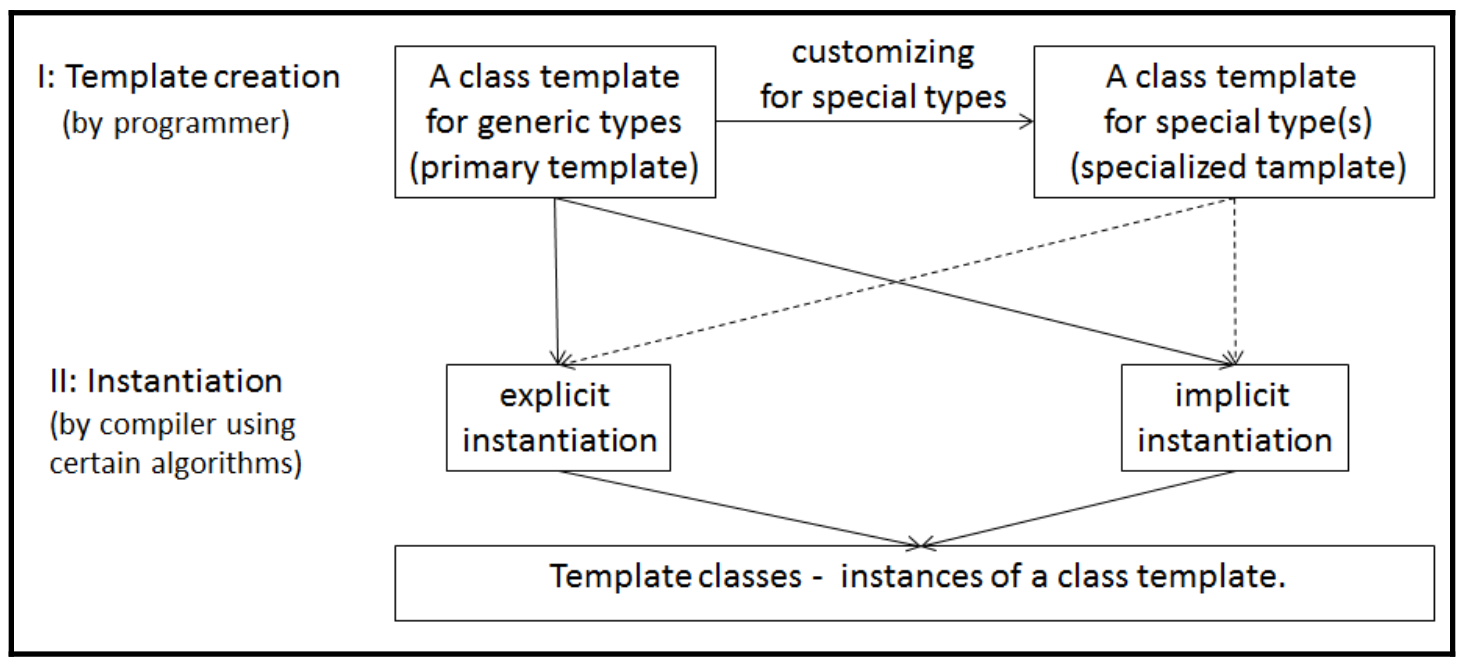
\includegraphics[width=0.6\textwidth]{content/Section-1/Chapter-4/2}
\end{center}

图的\textbf{I}中,使用特定的语法格式,可以为泛型类型创建类模板,也称为主模板,并且可以为具有不同成员函数和/或变量的特殊类型定制。\textbf{II}中,当我们有了类模板,编译器就会根据应用程序的需求显式或隐式地将模板实例化。\par
现在,了解一下创建类模板的语法。 \par

\noindent\textbf{}\ \par
\textbf{语法} \ \par
创建类模板的语法如下: \par

\begin{lstlisting}[caption={}]
[export] template <template_parameter_list> class-declaration
\end{lstlisting}

这里,我们有以下这些方式: \par

\begin{itemize}
	\item \texttt{template\underline{ }parameter-list}(请参扩展阅读中的链接)是一个非空的以逗号分隔的模板形参列表,每个模板形参要么是一个非类型形参,要么是一个类型形参,或是一个模板形参。
	\item \texttt{class-declaration}用来声明类,这个类包含一个类名和用花括号括起来的类体。通过这样做,声明的类名也变成了模板名。
\end{itemize}

例如,可以定义一个类模板V,使其包含各种1D数据类型:\par

\begin{lstlisting}[caption={}]
template <class T>
class V {
public:
	V( int n = 0) : m_nEle(n), m_buf(0) { creatBuf();}
	~V(){ deleteBuf(); }
	V& operator = (const V &rhs) { /* ... */}
	V& operator = (const V &rhs) { /* ... */}
	T getMax(){ /* ... */ }
protected:
	void creatBuf() { /* ... */}
	void deleteBuf(){ /* ... */}
public:
	int m_nEle;
	T * m_buf;
};
\end{lstlisting}

有了这个模板类,编译器就可以在实例化过程中生成类。由于在函数模板小节中提到的原因,本书中我们将避免使用不精确的术语定义模板类。 \par

\noindent\textbf{}\ \par
\textbf{实例化} \ \par
回顾一下上一节定义的类模板V,假设后面会出现以下声明: \par

\begin{lstlisting}[caption={}]
V<char> cV;
V<int> iV(10);
V<float> fV(5);
\end{lstlisting}

然后,编译器将创建V类的三个实例,如下所示: \par

\begin{lstlisting}[caption={}]
class V<char>{
public:
	V(int n=0);
	// ...
public:
	int m_nEle;
	char *m_buf;
};
class V<int>{
public:
	V(int n=0);
	// ...
public:
	int m_nEle;
	int *m_buf;
};
class V<float>{
public:
	V(int n = 0);
	// ...
public:
	int m_nEle;
	float *m_buf;
};
\end{lstlisting}

与函数模板实例化类似,类模板实例化有两种形式:显式和隐式。 \par

\noindent\textbf{}\ \par
\textbf{显式实例化} \ \par
显式实例化的语法如下: \par

\begin{lstlisting}[caption={}]
template class template_name < argument_list >;
extern template class template_name < argument_list >;//(since C++11)
\end{lstlisting}

显式实例化定义强制实例化的所引用的类、结构体或联合体。C++11标准中,模板特化或其成员的隐式实例化将被抑制。与函数模板的显式实例化类似,该显式实例化的位置可以在其模板定义之后的任何位置,并且只允许在整个程序的一个文件中定义。\par
而且,由于C++11隐式实例化将显式的声明(extern模板)绕过。这可以用来减少编译时间。 \par 
回到模板类V,我们可以显式地实例化它: \par

\begin{lstlisting}[caption={}]
template class V<int>;
template class V<double>;
\end{lstlisting}

或者,我们可以这样做(从C++11开始): \par

\begin{lstlisting}[caption={}]
extern template class V<int>;
extern template class V<double>;
\end{lstlisting}

如果显式实例化一个函数或类模板,但在程序中没有相应的定义,编译器将报出错误消息,如下所示: \par

\begin{lstlisting}[caption={}]
//ch4_4_class_template_explicit.cpp
#include <iostream>
using namespace std;
template <typename T> //line A
struct A {
	A(T init) : val(init) {}
	virtual T foo();
	T val;
}; //line B
//line C
template <class T> //T in this line is template parameter
T A<T>::foo() { //the 1st T refers to function return type,
	//the T in <> specifies that this function's template
	//parameter is also the class template parameter
	return val;
} //line D
extern template struct A<int>; //line E
#if 0 //line F
int A<int>::foo() {
	return val+1;
}
#endif //line G
int main(void) {
	A<double> x(5);
	A<int> y(5);
	cout<<"fD="<<x.foo()<<",fI="<<y.foo()<< endl;
	return 0; //output: fD=5,fI=6
}
\end{lstlisting}

前面的代码中,在A行和B行之间定义了一个类模板,然后从C行到D行实现了成员函数foo()。接下来,在E行为int类型显式实例化。由于在F行和G行之间的代码块注释掉了(这意味着对于这个显式的int类型实例化没有相应的foo()定义),我们有看到了链接错误。为了解决这个问题,我们需要在F行用\texttt{\#if 1}替换\texttt{\#if 0}。\par
最后,对于显式实例化声明还有一些限制: \par

\begin{itemize}
	\item \textbf{静态函数}:可以命名静态类成员,但不能在显式实例化声明中指定静态函数。
	\item \textbf{内联函数}:显式实例化声明中对内联函数没有影响,而内联函数是隐式实例化的。
	\item \textbf{类及其成员}:显式实例化类及其所有成员并不等价。
\end{itemize}

\noindent\textbf{}\ \par
\textbf{隐式实例化} \ \par
引用模板类时,编译器会在模板没有显式实例化或特化的情况下,按需生成代码,这称为隐式实例化: \par

\begin{lstlisting}[caption={}]
class_name<argument list> object_name; //for non-pointer object
class_name<argument list> *p_object_name; //for pointer object
\end{lstlisting}

对于非指针对象,实例化模板类并创建对象,只生成该对象使用的成员函数。对于指针对象,除非使用了其成员,否则不会实例化。 \par
以下示例中,我们在ch4\underline{ }5\underline{ }class\underline{ }template\underline{ }implicit\underline{ }insta.h文件中定义了一个类模板X:\par

\begin{lstlisting}[caption={}]
//file ch4_5_class_template_implicit_inst.h
#ifndef __CH4_5_H__
#define __CH4_5_H__
#include <iostream>
template <class T>
class X {
public:
	X() = default;
	~X() = default;
	void f() { std::cout << "X::f()" << std::endl; };
	void g() { std::cout << "X::g()" << std::endl; };
};
#endif
\end{lstlisting}

然后,它包含在以下四个cpp文件中,每个cpp文件中都有main()函数: \par

\begin{lstlisting}[caption={}]
//file ch4_5_class_template_implicit_inst_A.cpp
#include "ch4_5_class_template_implicit_inst.h"
void main()
{
	//implicit instantiation generates class X<int>, then create object xi
	X<int> xi ;
	//implicit instantiation generates class X<float>, then create object
	xf
	X<float> xf;
	return 0;
}
\end{lstlisting}

在ch4\underline{ }5\underline{ }class\underline{ }template\underline{ }implicit\underline{ }inst\underline{ }A.cpp中,编译器将隐式实例化X<int>和X<float>类,然后创建xi和xf对象。但是因为X::f()和X::g()没有使用,所以其实是没有实例化的。 \par
现在,来看看ch4\underline{ }5\underline{ }class\underline{ }template\underline{ }implicit\underline{ }inst\underline{ }B.cpp: \par

\begin{lstlisting}[caption={}]
//file ch4_5_class_template_implicit_inst_B.cpp
#include "ch4_5_class_template_implicit_inst.h"
void main()
{
	//implicit instantiation generates class X<int>, then create object xi
	X<int> xi;
	xi.f(); //and generates function X<int>::f(), but not X<int>::g()
	//implicit instantiation generates class X<float>, then create object
	//xf and generates function X<float>::g(), but not X<float>::f()
	X<float> xf;
	xf.g() ;
}
\end{lstlisting}

译器将隐式实例化X<int>类,创建xi对象,然后生成X<int>::f()函数,但不生成X<int>::g()。类似地,它将实例化X<float>类,创建xf对象,并生成X<float>::g()函数,但不生成X<float>::f()。 \par
然后,是ch4\underline{ }5\underline{ }class\underline{ }template\underline{ }implicit\underline{ }inst\underline{ }C.cpp: \par

\begin{lstlisting}[caption={}]
//file ch4_5_class_template_implicit_inst_C.cpp
#include "ch4_5_class_template_implicit_inst.h"
void main()
{
	//inst. of class X<int> is not required, since p_xi is pointer object
	X<int> *p_xi ;
	//inst. of class X<float> is not required, since p_xf is pointer object
	X<float> *p_xf ;
}
\end{lstlisting}

因为p\underline{ }xi和p\underline{ }xf是指针对象,所以不需要通过编译器实例化它们。 \par
最后是ch4\underline{ }5\underline{ }class\underline{ }template\underline{ }implicit\underline{ }inst\underline{ }D.cpp : \par

\begin{lstlisting}[caption={}]
//file ch4_5_class_template_implicit_inst_D.cpp
#include "ch4_5_class_template_implicit_inst.h"
void main()
{
	//inst. of class X<int> is not required, since p_xi is pointer object
	X<int> *p_xi;
	
	//implicit inst. of X<int> and X<int>::f(), but not X<int>::g()
	p_xi = new X<int>();
	p_xi->f();
	
	//inst. of class X<float> is not required, since p_xf is pointer object
	X<float> *p_xf;
	p_xf = new X<float>();//implicit inst. of X<float> occurs here
	p_xf->f(); //implicit inst. X<float>::f() occurs here
	p_xf->g(); //implicit inst. of X<float>::g() occurs here
	
	delete p_xi;
	delete p_xf;
}
\end{lstlisting}

这会隐式实例化X<int>和X<int>::f(),但不实例化X<int>::g()。X<float>,X<float>::f()和X<float>::g()也会实例化。 \par

\noindent\textbf{}\ \par
\textbf{特化} \ \par
与函数特化类似,当特定类型作为模板形参传递时,类模板的显式特化定义了不同的实现。然而,它仍然是一个类模板,需要通过实例化来获得真正的代码。\par
例如,假设有一个struct X模板,它可以存储任何数据类型的元素,并且它只有一个名为increase()的成员函数。但是对于char类型的数据,需要increase()有不同的实现,并需要向其添加一个名为toUpperCase()的新成员函数。因此,我们为该类型声明一个类模板的特化: \par

\begin{enumerate}
	\item 声明一个主类模板: \par
	\begin{lstlisting}[caption={}]
	template <typename T>
	struct X {
		X(T init) : m(init) {}
		T increase() { return ++m; }
		T m;
	};
	\end{lstlisting}
	声明了一个主类模板,它的构造函数初始化m成员变量,increase()给m加1并返回它的值。 \par
	\item 接下来,我们需要对char类型数据进行特化:  \par
	\begin{lstlisting}[caption={}]
	template <> //Note: no parameters inside <>, it tells compiler
	//"hi i am a fully specialized template"
	struct X<char> { //Note: <char> after X, tells compiler
		// "Hi, this is specialized only for type char"
		X(char init) : m(init) {}
		char increase() { return (m<127) ? ++m : (m=-128); }
		char toUpperCase() {
			if ((m >= 'a') && (m <= 'z')) m += 'A' - 'a';
			return m;
		}
		char m;
	};
	\end{lstlisting}
	创建一个特化的(相对于主类模板)类模板,多带有一个成员函数toUpperCase(),仅用于char类型数据。 \par
	\item 现在,运行一个测试:   \par
	\begin{lstlisting}[caption={}]
	int main() {
		X<int> x1(5); //line A
		std::cout << x1.increase() << std::endl;
		X<char> x2('b'); //line B
		std::cout << x2.toUpperCase() << std::endl;
		return 0;
	}
	\end{lstlisting}
\end{enumerate}

最后,用一个main()函数来测试它。第A行,x1是一个从主模板X<t>隐式实例化的对象。因为x1的初始值。m是5,6将从x1.increase()返回。第B行,x2是从特化模板X<char>和x2的值实例化的对象。m在执行时是‘b’,在调用x2.toUpperCase()之后,‘B’将是返回值。 \par

\hspace*{\fill} \\ %插入空行

\includegraphics[width=0.05\textwidth]{images/tip}
可以在ch4\underline{ }6\underline{ }class\underline{ }template\underline{ }specialization.cpp看到这个示例的完整代码。 \par
\noindent\textbf{}\ \par

总之,类模板的显式特化中的使用方式如下所示: \par

\begin{lstlisting}[caption={}]
template <> class[struct] class_name<template argument list> { ... };
\end{lstlisting}

这里,空的模板形参表template <>显式地声明为模板特化,<目标参数列表>是要特化的类型形参。例如,在ex4\underline{ }6\underline{ }class\underline{ }template\underline{ }specialize.cpp中,使用以下方法: \par

\begin{lstlisting}[caption={}]
template <> struct X<char> { ... };
\end{lstlisting}

这里,X之后的<char>标识了要为其声明模板类特化的类型。\par
此外,在对模板类进行特化时,必须定义所有成员(甚至主模板中相同的成员),因为在模板特化期间,没有继承主模板。 \par
接下来,我们将研究部分特化。这是显式专门化的一般表达。与只有模板实参列表的显式特化相比,部分特化同时需要模板形参列表和实参列表。对于模板实例化,如果用户的模板实参列表匹配模板实参的子集,编译器将选择部分特化模板。然后,编译器将生成来部分特化模板的类定义。 \par
下面的例子中,对于主类模板A,可以在实参列表中为const T部分特化它。注意,它们都有相同的参数列表,即<typename T>: \par

\begin{lstlisting}[caption={}]
//primary class template A
template <typename T> class A{ /* ... */ };

//partial specialization for const T
template <typename T> class A<const T>{ /* ... */ };
\end{lstlisting}

下面的示例中,主类模板B有两个参数:<typename T1,typename T2>。我们通过T1=int部分特化它,保持T2不变: \par

\begin{lstlisting}[caption={}]
//primary class template B
template <typename T1, typename T2> class B{ /* ... */ };

//partial specialization for T1 = int
template <typename T2> class B<int, T2>{ /* ... */};
\end{lstlisting}

最后,在下面的示例中,可以看到部分特化中的模板形参数量不必与原始主模板中出现的形参数量匹配。但是,模板实参的数量(出现在尖括号中的类名之后)必须与主模板中的形参的数量和类型匹配: \par

\begin{lstlisting}[caption={}]
//primary class template C: template one parameter
template <typename T> struct C { T type; };

//specialization: two parameters in parameter list
//but still one argument (<T[N]>) in argument list
template <typename T, int N> struct C<T[N]>
{T type; };
\end{lstlisting}

同样,模板类的部分特化仍然是模板类。必须分别为其成员函数和数字变量提供定义。\par
我们总结一下到目前为止所学的内容。下表中,可以看到函数模板和类模板的比较:\par

\begin{table}[h]
	\begin{tabularx}{\textwidth}{|p{2cm}|X|X|X|}
		\hline
		& 函数模板  & 模板类  & 注释 \\ 
		\hline
		声明	& \texttt{template <class T1, class T2> void f(T1 a, T2 b){ ... }} & \texttt{template <class T1, class T2> class X { ...};} & 声明中定义了一个函数/类模板,\texttt{<class T1,class T2>}称为模板形参。 \\
		\hline
		显式实例化 & \texttt{template void f<int, int >( int, int);}或 \texttt{extern template	void f <int, int>( int, int); // (since C++11)} & \texttt{template class X<int, float>;} 或 \texttt{extern template	class X<int,float>; //(since C++11)} & 在实例化之后,现在有函数/类,但它们叫做模板函数/类。 \\
		\hline
		隐式实例化	& \texttt{\{
			... 
			f(3, 4.5);
			f<char,
			float>(120, 3.14);
		\}} & \texttt{\{
			... 
			X<int,float> obj; 
			X<char, char> *p;
		\}} & 当函数调用或类对象/指针声明时,如果没有显式实例化,则使用隐式实例化。 \\
		\hline
		特化	& \texttt{template <> void f<int,float>(int a, float b){ ... }} & \texttt{template <> class X <int, float>{ ... };} & 主模板的完全定制版本(没有参数列表)仍然需要实例化。 \\
		\hline
		部分特化	& \texttt{template <class T> void f<T,T>(T a, T b) { ... }} & \texttt{template <class T> class X <T, T>{	... };} & 主模板的部分定制版本(有一个参数列表)仍然需要实例化。 \\ 
		\hline
	\end{tabularx}
\end{table}

这里需要强调五个概念: \par

\begin{itemize}
	\item \textbf{声明}:需要遵循定义函数或模板类的语法。此时,函数或模板类本身就不是类型、函数或其他实体。换句话说,源文件中只有模板定义,而没有可以编译为目标文件的代码。
	\item \textbf{隐式实例化}:对于任何代码,模板必须实例化。此过程中,必须确定模板参数,以便编译器能够生成实际的函数或类。换句话说,这是按需编译的,在给出带有特定模板参数的实例化之前,不会编译模板函数或类的代码。
	\item \textbf{显式实例化}:告诉编译器使用给定类型实例化模板,而不管是否使用了这些类型。通常,用于提供库。
	\item \textbf{全特化}:没有模板参数列表(完全定制)。模板特化最有用的一点是可以为特定的类型参数创建特定的模板。
	\item \textbf{部分特化}:与全特化类似,但是只有部分形参(部分定制)和部分实参。
\end{itemize}

\noindent\textbf{}\ \par
\textbf{了解可变模板} \ \par
上一节中,学习了如何编写固定数量类型参数的函数或类模板。不过,自C++11以来,标准泛型函数和类模板可以接受数量可变的类型参数,这称为可变参数模板,C++在进一步读取上下文中的扩展。我们将通过示例,了解可变参数模板的语法和用法。 \par

\noindent\textbf{}\ \par
\textbf{语法} \ \par
如果函数或模板类接受零个或多个形参,则可以如下定义: \par

\begin{lstlisting}[caption={}]
//a class template with zero or more type parameters
template <typename... Args> class X { ... };

//a function template with zero or more type parameters
template <typename... Args> void foo( function param list) { ...}
\end{lstlisting}

在这里,\texttt{<typename ... Args>}声明了一个参数包。注意,这里Args不是关键字,可以使用任何有效的变量名对其进行替换。前面的模板类/函数可以接受任意数量的typename,作为实例化的参数,如下所示: \par

\begin{lstlisting}[caption={}]
X<> x0; //with 0 template type argument
X<int, std::vector<int> > x1; //with 2 template type arguments

//with 4 template type arguments
X<int, std::vector<int>, std::map<std::string, std::vector<int>>> x2;

//with 2 template type arguments
foo<float, double>( function argument list );

//with 3 template type arguments
foo<float, double, std::vector<int>>( function argument list );
\end{lstlisting}

如果可变参数模板至少需要一个类型形参,可以使用以下定义: \par

\begin{lstlisting}[caption={}]
template <typename A, typename... Rest> class Y { ... };

template <typename A, typename... Rest>
void goo( const int a, const float b) { ....};
\end{lstlisting}

类似地,可以使用下面的代码来实例化它们: \par

\begin{lstlisting}[caption={}]
Y<int > y1;
Y<int, std::vector<int>, std::map<std::string, std::vector<int>>> y2;
goo<int, float>( const int a, const float b );
goo<int,float, double, std::vector<int>>( const int a, const float b );
\end{lstlisting}

代码中,使用variadic类模板Y的实例化中创建了y1和y2对象,分别带有一个和三个模板参数。对于可变参数函数goo模板,将其实例化为两个模板函数,分别带有两个和三个模板参数。 \par

\noindent\textbf{}\ \par
\textbf{例子} \ \par
下面可能是最简单的例子,展示了使用可变参数模板来查找任何输入参数列表的最小值。这个例子使用了递归,直到my\underline{ }min(double n)时退出迭代: \par

\begin{lstlisting}[caption={}]
//ch4_7_variadic_my_min.cpp
//Only tested on g++ (Ubuntu/Linaro 7.3.0-27 ubuntu1~18.04)
//It may have compile errors for other platforms
#include <iostream>
#include <math.h>
double my_min(double n){
	return n;
}
template<typename... Args>
double my_min(double n, Args... args){
	return fmin(n, my_min(args...));
}
int main() {
	double x1 = my_min(2);
	double x2 = my_min(2, 3);
	double x3 = my_min(2, 3, 4, 5, 4.7,5.6, 9.9, 0.1);
	std::cout << "x1="<<x1<<", x2="<<x2<<", x3="<<x3<<std::endl;
	return 0;
}
\end{lstlisting}

printf()变参数函数可能是C和C++中最有用和最强大的函数。然而,它不是类型安全的。在下面的代码块中,我们将采用类型安全的printf()示例来演示可变参数模板的用法。和往常一样,首先定义一个基函数\texttt{void printf\underline{ }vt(const char *s)},以结束递归: \par

\begin{lstlisting}[caption={}]
//ch4_8_variadic_printf.cpp part A: base function - recursive end
void printf_vt(const char *s)
{
	while (*s){
		if (*s == '%' && *(++s) != '%')
		throw std::runtime_error("invalid format string: missing arguments");
		std::cout << *s++;
	}
}
\end{lstlisting}

然后,它的可变参数模板函数printf\underline{ }vt()中,每当有\%时,该值就会打印出来,其余的则传递给它的递归,直到基函数为止: \par

\begin{lstlisting}[caption={}]
//ch4_8_variadic_printf.cpp part B: recursive function
template<typename T, typename... Rest>
void printf_vt(const char *s, T value, Rest... rest)
{
	while (*s) {
		if (*s == '%' && *(++s) != '%') {
			std::cout << value;
			printf_vt(s, rest...); //called even when *s is 0,
			return; //but does nothing in that case
		}
		std::cout << *s++;
	}
}
\end{lstlisting}

最后,可以使用下面的代码来测试它,并将其与传统的printf()进行比较: \par

\begin{lstlisting}[caption={}]
//ch4_8_variadic_printf.cpp Part C: testing
int main() {
	int x = 10;
	float y = 3.6;
	std::string s = std::string("Variadic templates");
	const char* msg1 = "%s can accept %i parameters (or %s), x=%d, y=%f\n";
	printf(msg1, s, 100, "more",x,y); //replace 's' by 's.c_str()'
	//to prevent the output bug
	const char* msg2 = "% can accept % parameters (or %); x=%,y=%\n";
	printf_vt(msg2, s, 100, "more",x,y);
	return 0;
}
\end{lstlisting}

上述代码的输出如下: \par

\begin{lstlisting}[caption={}]
p.]�U can accept 100 parameters (or more), x=10, y=3.600000
Variadic templates can accept 100 parameters (or more); x=10,y=3.6
\end{lstlisting}

第一行的开始,可以看到printf()中的一些ASCII字符,因为对应的变量类型\%s应该是一个指向char的指针,但我们给它指定了std::string类型。要解决这个问题,需要传递s.c\underline{ }str()。然而,有了可变参数版本函数,就没有这个问题了。此外,只需要提供\%,就好了——至少对于这个实现来说是这样的。 \par

总之,本节简要介绍了可变参数模板及其应用。可变参数模板有以下优点(自C++ 11以来): \par

\begin{itemize}
	\item 模板的轻量级扩展
	\item 演示了在不使用模板和预处理宏的情况下实现模板库的能力。因此,代码能够理解和调试,同时也节省了编译时间。
	\item 支持printf()可变参数函数的类型安全实现。
\end{itemize}

接下来,我们将探讨模板形参和参数。\par

\noindent\textbf{}\ \par
\textbf{探索模板形参和参数} \ \par
前两节中学习了函数和模板类以及它们的实例化。在定义模板时,需要给出形参列表。当实例化时,必须提供相应的参数列表。本节中,将进一步研究这两个列表的分类和细节。 \par

\noindent\textbf{}\ \par
\textbf{模板参数} \ \par
回想一下下面的语法,它是用来定义模板类/函数的。模板关键字后面有一个<>符号,必须给出一个或多个模板形参: \par

\begin{lstlisting}[caption={}]
//class template declaration
template <parameter-list> class-declaration

//function template declaration
template <parameter-list> function-declaration
\end{lstlisting}

形参列表中的可以是以下三种类型之一: \par

\begin{itemize}
	\item 非类型模板形参:指引用静态实体的编译时常量值,如整数和指针。这些参数通常称为非类型参数。 
	\item 类型模板形参:它引用内置类型名或用户定义的类。
	\item 模板的模板参数:表示该参数为其他模板。
\end{itemize}

我们将在下面的小节中更详细地讨论这些问题。 \par

\noindent\textbf{}\ \par
\textbf{非类型模板参数} \ \par
非类型模板形参的语法如下: \par

\begin{lstlisting}[caption={}]
//for a non-type template parameter with an optional name
type name(optional)

//for a non-type template parameter with an optional name
//and a default value
type name(optional)=default

//For a non-type template parameter pack with an optional name
type ... name(optional) (since C++11)
\end{lstlisting}

这里,类型是以下类型之一——整型、枚举、指向对象或函数的指针、指向对象或函数的左值引用、指向成员对象或成员函数的指针,以及std::nullptr\underline{ }t(C++11)。此外,可以在模板声明中放入数组和/或函数类型,它们会被数据和/或函数指针自动替换。 \par
下面的示例显示了一个使用非类型模板形参int N的类模板。main()中实例化并创建了一个对象x,因此x.a有五个初始值为1的元素。将第四个元素的值设置为10之后,输出结果:\par

\begin{lstlisting}[caption={}]
//ch4_9_none_type_template_param1.cpp
#include <iostream>
template<int N>
class V {
	public:
	V(int init) {
		for (int i = 0; i<N; ++i) { a[i] = init; }
	}
	int a[N];
};
int main()
{
	V<5> x(1); //x.a is an array of 5 int, initialized as all 1's
	x.a[4] = 10;
	for( auto &e : x.a) {
		std::cout << e << std::endl;
	}
}
\end{lstlisting}

下面是使用const char*作为非类型模板形参的函数模板示例: \par

\begin{lstlisting}[caption={}]
//ch4_10_none_type_template_param2.cpp
#include <iostream>
template<const char* msg>
void foo() {
	std::cout << msg << std::endl;
}
// need to have external linkage
extern const char str1[] = "Test 1";
constexpr char str2[] = "Test 2";
extern const char* str3 = "Test 3";
int main()
{
	foo<str1>(); //line 1
	foo<str2>(); //line 2
	//foo<str3>(); //line 3
	const char str4[] = "Test 4";
	constexpr char str5[] = "Test 5";
	//foo<str4>(); //line 4
	//foo<str5>(); //line 5
	return 0;
}
\end{lstlisting}

main()中成功地用str1和str2实例化了foo(),它们都是编译时常量值,并且具有外部链接。如果取消注释第3-5行,编译器将报告错误消息。得到这些编译错误的原因如下: \par

\begin{itemize}
	\item Line 3:  str3不是const变量,因此不能更改str3所指向的值。str3的值可以修改。
	\item Line 4:  str4不是const char*类型的有效模板实参,因为它没有链接。
	\item Line 5:  str5不是const char*类型的有效模板实参,因为它没有链接。
\end{itemize}

非类型形参的另一种最常见用法是使用数组的大小。如果你想了解更多,请访问\\ https://stackoverflow.com/questions/​33234979 

\noindent\textbf{}\ \par
\textbf{模板参数类型} \ \par
type模板形参的语法如下: \par

\begin{lstlisting}[caption={}]
//A type Template Parameter (TP) with an optional name
typename |class name(optional)

//A type TP with an optional name and a default
typename[class] name(optional) = default

//A type TP pack with an optional name
typename[class] ... name(optional) (since C++11)
\end{lstlisting}

\hspace*{\fill} \\ %插入空行

\includegraphics[width=0.05\textwidth]{images/tip}
注意:这里,typename和class关键字可以互换。模板声明体中,类型参数的名称是typedef-name。当模板实例化时,为类型提供别名。 \par
\noindent\textbf{}\ \par

现在,让我们来看一些例子: \par

\begin{itemize}
	\item 没有默认值的类型模板参数: \par
	\begin{lstlisting}[caption={}]
	Template<class T> //with name
	class X { /* ... */ };
	
	Template<class > //without name
	class Y { /* ... */ };
	\end{lstlisting}
	\item 默认的类型模板参数: \par
	\begin{lstlisting}[caption={}]
	Template<class T = void> //with name
	class X { /* ... */ };
	
	Template<class = void > //without name
	class Y { /* ... */ };
	\end{lstlisting}
	\item 类型模板参数包: \par
	\begin{lstlisting}[caption={}]
	template<typename... Ts> //with name
	class X { /* ... */ };
	
	template<typename... > //without name
	class Y { /* ... */ };
	\end{lstlisting}
\end{itemize}

模板形参包可以接受零个或多个模板形参,并且只在C++11以后有效。 \par

\noindent\textbf{}\ \par
\textbf{模板的模板参数} \ \par
模板参数template的语法如下: \par

\begin{lstlisting}[caption={}]
//A template template parameter with an optional name
template <parameter-list> class name(optional)

//A template template parameter with an optional name and a default
template <parameter-list> class name(optional) = default

//A template template parameter pack with an optional name
template <parameter-list> class ... name(optional) (since C++11)
\end{lstlisting}

\hspace*{\fill} \\ %插入空行

\includegraphics[width=0.05\textwidth]{images/tip}
注意:模板参数的形参声明中,只能使用class关键字,不允许使用typename。在模板声明的主体中,形参的名称是模板名,需要实参来实例化。\par
\noindent\textbf{}\ \par

假设你有一个函数,作为对象列表的流输出操作符: \par

\begin{lstlisting}[caption={}]
template<typename T>
static inline std::ostream &operator << ( std::ostream &out,
std::list<T> const& v)
{
	/*...*/
}
\end{lstlisting}

前面的代码中可以看到,对于序列容器(如数组、双端队列和多种映射类型)是相同的。因此,使用template模板形参的概念,可以使用操作符<<来规则所有这些。例子可以在exch4\underline{ }tp\underline{ }c.cpp中找到:\par

\begin{lstlisting}[caption={}]
//ch4_11_template_template_param.cpp (courtesy: https:/​/​stackoverflow.​com/
questions/​213761)
#include <iostream>
#include <vector>
#include <deque>
#include <list>

using namespace std;
template<class T, template<class, class...> class X, class... Args>
std::ostream& operator <<(std::ostream& os, const X<T, Args...>& objs) {
	os << __PRETTY_FUNCTION__ << ":" << endl;
	for (auto const& obj : objs)
	os << obj << ' ';
	return os;
}

int main() {
	vector<float> x{ 3.14f, 4.2f, 7.9f, 8.08f };
	cout << x << endl;
	list<char> y{ 'E', 'F', 'G', 'H', 'I' };
	cout << y << endl;
	deque<int> z{ 10, 11, 303, 404 };
	cout << z << endl;
	return 0;
}
\end{lstlisting}

上述程序的输出如下所示:

\begin{lstlisting}[caption={}]
class std::basic_ostream<char,struct std::char_traits<char> > &__cdecl
operator
<<<float,class std::vector,class std::allocator<float>>(class
std::basic_ostream
<char,struct std::char_traits<char> > &,const class std::vector<float,class
std:
:allocator<float> > &):
3.14 4.2 7.9 8.08
class std::basic_ostream<char,struct std::char_traits<char> > &__cdecl
operator
<<<char,class std::list,class std::allocator<char>>(class
std::basic_ostream<cha
r,struct std::char_traits<char> > &,const class std::list<char,class
std::alloca
tor<char> > &):
E F G H I
class std::basic_ostream<char,struct std::char_traits<char> > &__cdecl
operator
<<<int,class std::deque,class std::allocator<int>>(class
std::basic_ostream<char
,struct std::char_traits<char> > &,const class std::deque<int,class
std::allocat
or<int> > &):
10 11 303 404	
\end{lstlisting}

如预期的那样,每次调用的输出的第一部分是模板函数名,而第二部分则输出每个容器的元素值。 \par

\noindent\textbf{}\ \par
\textbf{模板参数} \ \par
实例化一个模板,所有的模板形参必须用它们对应的模板形参替换。实参要么显式提供,要么从初始化式推导(对于类模板),要么从上下文推导(对于函数模板),或有默认值。由于有三种类型的模板形参,我们也将有三个相应的模板形参。它们是模板非类型实参、模板类型实参和模板模板实参。除此之外,我们还将讨论默认的模板实参。 \par

\noindent\textbf{}\ \par
\textbf{模板非类型参数} \ \par
回想一下,非类型模板形参引用的是编译时常量值,比如:整数、指针和对静态实体的引用。模板参数列表中提供的非类型模板参数必须与这些值匹配。通常,非类型模板实参用于类初始化或类容器的大小。 \par
虽然,详细的规则为讨论每个类型(整型和算术类型,指针/函数/对象成员,左值引用参数等)的实参数超出了本书的范畴,一般规则模板实参数应该转化为模板参数常数表达式。 \par
让我们来看看下面的例子: \par

\begin{lstlisting}[caption={}]
//part 1: define template with non-type template parameters
template<const float* p> struct U {}; //float pointer non-type parameter
template<const Y& b> struct V {}; //L-value non-type parameter
template<void (*pf)(int)> struct W {};//function pointer parameter

//part 2: define other related stuff
void g(int,float); //declare function g()
void g(int); //declare an overload function of g()
struct Y { //declare structure Y
	float m1;
	static float m2;
};
float a[10];
Y y; //line a: create a object of Y

//part 3: instantiation template with template non-type arguments
U<a> u1; //line b: ok: array to pointer conversion
U<&y> u2; //line c: error: address of Y
U<&y.m1> u3; //line d: error: address of non-static member
U<&y.m2> u4; //line e: ok: address of static member
V<y> v; //line f: ok: no conversion needed
W<&g> w; //line g: ok: overload resolution selects g(int)
\end{lstlisting}

前面第1部分的代码中,我们定义了三个具有不同非类型模板形参的模板结构。然后,第2部分中,声明了两个重载函数和结构体Y。最后,第3部分中,讨论了通过不同的非类型参数来实例化它们的正确方法。\par

\noindent\textbf{}\ \par
\textbf{模板类型的参数} \ \par
与模板的非类型实参相比,模板类型实参(用于类型模板形参)的规则很简单,必须是typeid。在这里,typeid是一个标准C++操作符,会在运行时返回类型标识信息。它返回一个type\underline{ }info对象,可以与其他type\underline{ }info对象进行比较。 \par
看看下面的例子: \par

\begin{lstlisting}[caption={}]
//ch4_12_template_type_argument.cpp
#include <iostream>
#include <typeinfo>
using namespace std;

//part 1: define templates
template<class T> class C {};
template<class T> void f() { cout << "T" << endl; };
template<int i> void f() { cout << i << endl; };

//part 2: define structures
struct A{}; // incomplete type
typedef struct {} B; // type alias to an unnamed type

//part 3: main() to test
int main() {
	cout << "Tid1=" << typeid(A).name() << "; ";
	cout << "Tid2=" << typeid(A*).name() << "; ";
	cout << "Tid3=" << typeid(B).name() << "; ";
	cout << "Tid4=" << typeid(int()).name() << endl;
	
	C<A> x1; //line A: ok,'A' names a type
	C<A*> x2; //line B: ok, 'A*' names a type
	C<B> x3; //line C: ok, 'B' names a type
	f<int()>(); //line D: ok, since int() is considered as a type,
				//thus calls type template parameter f()
	f<5>(); //line E: ok, this calls non-type template parameter f()
	return 0;
}
\end{lstlisting}

本例(第1部分)中,定义了三个类模板和函数模板:带有类型模板形参的类模板C,两个带有类型模板形参的函数模板,以及一个非类型模板形参。第2部分中,有一个不完整的结构体A和一个未命名的结构体B。最后,第3部分中,我们测试了它们。4个typeid()在Ubuntu 18.04中的输出如下: \par

\begin{lstlisting}[caption={}]
Tid1=A; Tid2=P1A; Tid3=1B; Tid4=FivE
\end{lstlisting}

x86的MSVC v19.24,会输出以下内容: \par

\begin{lstlisting}[caption={}]
Tid1=struct A; Tid2=struct A; Tid3=struct B; Tid4=int __cdecl(void)
\end{lstlisting}

另外,由于A、A*、B和int()都有typeid,所以从A行到D行的代码段与模板类型类或函数相链接。只有E行是从非类型模板形参函数模板实例化的,即f()。 \par

\noindent\textbf{}\ \par
\textbf{模板的模板参数} \ \par
对于模板模板形参,其对应的模板实参是类模板的名称或模板别名。寻找与模板参数匹配的模板时,只考虑主类模板。 \par
这里,主模板指的是特化的模板。即使它们的形参列表可能匹配,编译器也不会考虑使用模板形参的部分特化。 \par
下面是一个模板参数的例子: \par

\begin{lstlisting}[caption={}]
//ch4_13_template_template_argument.cpp
#include <iostream>
#include <typeinfo>
using namespace std;

//primary class template X with template type parameters
template<class T, class U>
class X {
	public:
	T a;
	U b;
};

//partially specialization of class template X
template<class U>
class X<int, U> {
	public:
	int a; //customized a
	U b;
};

//class template Y with template template parameter
template<template<class T, class U> class V>
class Y {
	public:
	V<int, char> i;
	V<char, char> j;
};

Y<X> c;
int main() {
cout << typeid(c.i.a).name() << endl; //int
cout << typeid(c.i.b).name() << endl; //char
cout << typeid(c.j.a).name() << endl; //char
cout << typeid(c.j.b).name() << endl; //char
return 0;
}
\end{lstlisting}

本例中,定义了一个主类模板X及其特化,然后定义了类模板Y,带有模板形参。接下来,我们用模板参数X隐式实例化Y,并创建一个对象c。最后,main()输出四个typeid()的名称,结果分别是int、char、char和char。 \par

\noindent\textbf{}\ \par
\textbf{默认模板参数} \ \par
C++中函数通过传递参数来调用,而参数由函数使用。如果在调用函数时没有传递参数,则使用默认值。与函数形参默认值类似,模板形参也可以有默认实参。定义模板时,可以设置它的默认实参,如下所示: \par

\begin{lstlisting}[caption={}]
//ch4_14_default_template_arguments.cpp //line 0
#include <iostream> //line 1
#include <typeinfo> //line 2
template<class T1, class T2 = int> class X; //line 3
template<class T1 = float, class T2> class X;//line 4
template<class T1, class T2> class X { //line 5
	public: //line 6
	T1 a; //line 7
	T2 b; //line 8
}; //line 9
using namespace std;
int main() {
	X<int> x1; //<int,int>
	X<float> x2; //<float,int>
	X<> x3; //<float,int>
	X<double, char> x4; //<double, char>
	cout << typeid(x1.a).name() << ", " << typeid(x1.b).name() << endl;
	cout << typeid(x2.a).name() << ", " << typeid(x2.b).name() << endl;
	cout << typeid(x3.a).name() << ", " << typeid(x3.b).name() << endl;
	cout << typeid(x4.a).name() << ", " << typeid(x4.b).name() << endl;
	return 0
}
\end{lstlisting}

为模板形参设置默认实参时,需要遵循以下规则: \par

\begin{itemize}
	\item 声明顺序很重要——默认模板实参的声明必须在主模板声明的顶部。例如,在前面的示例中,不能将第3行和第4行代码移到第9行之后。
	\item 如果一个形参有一个默认实参,那么它之后的所有形参也必须有默认实参。例如,以下代码是不正确的:
	\begin{lstlisting}[caption={}]
	template<class U = char, class V, class W = int> class X { }; //Error
	template<class V, class U = char, class W = int> class X { }; //OK
	\end{lstlisting}
	\item 不能在同一个作用域中两次给出相同的形参默认实参。例如,如果使用下面的代码,会得到一个错误消息:
	\begin{lstlisting}[caption={}]
	template<class T = int> class Y;
	
	//compiling error, to fix it, replace "<class T = int>" by "<class T>"
	template<class T = int> class Y {
		public: T a;
	};
	\end{lstlisting}
\end{itemize}

这里,讨论了两个列表:template\underline{ }parameter\underline{ }list和template\underline{ }argument\underline{ }list。它们分别用于函数或类模板的创建和实例化。\par
还要了解了另外两条重要的规则: \par

\begin{itemize}
	\item 定义模板类或函数时,需要给出它的template\underline{ }parameter\underline{ }list:
	\begin{lstlisting}[caption={}]
	template <template_parameter_list>
	class X { ... }
	
	template <template_parameter_list>
	void foo( function_argument_list ) { ... } //assume return type is void
	\end{lstlisting}
	\item 实例化时,必须提供相应的argument\underline{ }list:
	\begin{lstlisting}[caption={}]
	class X<template_argument_list> x
	void foo<template_argument_list>( function_argument_list )
	\end{lstlisting}
\end{itemize}

这两个列表中的形参或实参类型可以分为三类,如下表所示。注意,虽然第一行是模板类,但这些属性也适用于模板函数: \par

\begin{table}[h]
	\begin{tabularx}{\textwidth}{|p{2cm}|X|X|}
		\hline
		& 定义模板时 template <template\_parameter\_list> class X \{ ... \} & 实例化一个模板时class X<template\_argument\_list> x \\ 
		
		\hline
		非类型
		 & 
		该参数列表中的实体可以是下列类型之一:
		\begin{itemize}
			\item 整型或枚举
			\item 指向对象或函数的指针
			\item 对象的左值引用或函数的左值引用
			\item 成员指针
			\item C++11 std::nullptr\underline{ }t
		\end{itemize} & 
		\begin{itemize}
		\item 此列表中的非类型参数是表达式,其值可以在编译时确定。
		\item 这些参数必须是常量表达式、具有外部链接的函数或对象的地址,或静态类成员的地址。
		\item 非类型实参通常用于初始化类或指定类成员的大小。
		\end{itemize} \\
		\hline
		类型 
		& 
		该参数列表中的实体可以是下列类型之一:
		\begin{itemize}
			\item 必须以typename或class开始
			\item 在模板声明体中,类型的名称	
		\end{itemize} 
		参数是typedef-name。当模板实例化时,它为提供的类型提供别名。
		& 
		\begin{itemize}
			\item 参数的类型必须有一个typeid
			\item 不能是局部类型、没有链接的类型、未命名类型或由任何这些类型复合而成的类型。
		\end{itemize} \\
		\hline
		模板 
		& 
		该参数列表中的实体可以是下列类型之一:
		\begin{itemize}
			\item template <parameter-list> class name
			\item template <parameter-list> class ... name
			(可选) (C++11)
		\end{itemize} 
		& 
		列表中的模板参数是类模板的名称 \\
		\hline
	\end{tabularx}
\end{table}

\newpage

下一节中,我们将探索如何用C++实现特征,并使用它们优化算法。 \par

\noindent\textbf{}\ \par
\textbf{探索特征} \ \par
泛型编程需要编写在特定需求下,适用于任何数据类型的代码。这是在软件工程行业中交付可重用高质量代码的最有效的方法。然而,在泛型编程中,有时泛型还不够好。当类型之间的差异过于复杂时,高效泛型很难通用化实现。例如,实现sort函数模板时,如果知道参数类型是链表而不是数组,那么将实现不同的策略来优化性能。 \par
尽管模板特化是克服这个问题的方法,但并没有以广泛的方式提供与类型相关的信息。类型特征是一种用来收集类型信息的技术。我们可以做出更智能的决策,开发高质量的泛型编程优化算法。 \par
本节中,我们将介绍如何实现类型特征,然后展示如何使用类型信息来优化算法。 \par

\noindent\textbf{}\ \par
\textbf{类型特征实现} \ \par
为了理解类型特征,来看看boost::is\underline{ }void和boost::is\underline{ }pointer的实现。\par

\noindent\textbf{}\ \par
\textbf{boost::is\underline{ }void} \ \par
首先,看一个最简单的trait类,is\underline{ }void特征是由boost创建的,定义了一个用于实现默认行为的通用模板,接受一个空类型,但其他类型都为空。因此,可得到\texttt{is\underline{ }void::value = false}: \par

\begin{lstlisting}[caption={}]
//primary class template is_void
template< typename T >
struct is_void{
	static const bool value = false; //default value=false
};
\end{lstlisting}

然后,我们对void类型进行完全特化:\par

\begin{lstlisting}[caption={}]
//"<>" means a full specialization of template class is_void
template<>
struct is_void< void >{ //fully specialization for void
	static const bool value = true; //only true for void type
};
\end{lstlisting}

这样,我们就有了一个完整的traits类型,可以通过检查以下表达式,来检测给定类型T是否为void: \par

\begin{lstlisting}[caption={}]
is_void<T>::value
\end{lstlisting}

接下来,了解下如何在boost::is\underline{ }pointer中使用部分特化。 \par

\noindent\textbf{}\ \par
\textbf{boost::is\underline{ }pointer} \ \par
与boost::avoid特征类似,主类模板的定义如下:\par

\begin{lstlisting}[caption={}]
//primary class template is_pointer
template< typename T >
struct is_pointer{
	static const bool value = false;
};
\end{lstlisting}

然后,部分特化所有指针类型: \par

\begin{lstlisting}[caption={}]
//"typename T" in "<>" means partial specialization
template< typename T >
struct is_pointer< T* >{ //<T*> means partial specialization only for type
	T*
	static const bool value = true; //set value as true
};
\end{lstlisting}

现在,我们有了一个完整的特征类型,可以通过检查以下表达式来检测给定类型T是否指针: \par

\begin{lstlisting}[caption={}]
is_pointer<T>::value
\end{lstlisting}

由于boost类型特征特性已经正式加入到C++11标准库中,我们可以在以下示例中展示std::is\underline{ }void和std::is\underline{ }pointer的用法,而不需要包含前面示例中的源代码: \par

\begin{lstlisting}[caption={}]
//ch4_15_traits_boost.cpp
#include <iostream>
#include <type_traits> //since C++11
using namespace std;
struct X {};
int main()
{
	cout << boolalpha; //set the boolalpha format flag for str stream.
	cout << is_void<void>::value << endl; //true
	cout << is_void<int>::value << endl; //false
	cout << is_pointer<X *>::value << endl; //true
	cout << is_pointer<X>::value << endl; //false
	cout << is_pointer<X &>::value << endl; //false
	cout << is_pointer<int *>::value << endl; //true
	cout << is_pointer<int **>::value << endl; //true
	cout << is_pointer<int[10]>::value << endl; //false
	cout << is_pointer< nullptr_t>::value << endl; //false
}
\end{lstlisting}

代码在开头为字符串流设置了boolalpha格式标记。通过这样做,所有的bool值都通过它们的文本表示来提取,文本表示为真或假。然后,使用std::cout来打印is\underline{ }void<t>::value和is\underline{ }pointer<t>::value的值。每个值的输出显示在相应行的末尾注释中。 \par

\noindent\textbf{}\ \par
\textbf{利用特征优化算法} \ \par
我们将使用一个优化复制的示例,来展示类型特征的用法,而不是通过的抽象方式来讨论。使用标准库中的copy算法: \par

\begin{lstlisting}[caption={}]
template<typename It1, typename It2>
It2 copy(It1 first, It1 last, It2 out);
\end{lstlisting}

显然,可以为任何类型的迭代器编写copy()的泛型版本,即这里的It1和It2。然而,正如boost库作者所说的的那样,某些情况下,memcpy()可以执行复制操作。如果满足以下所有条件,就可以使用memcpy():\par

\begin{itemize}
	\item It1和It2这两种类型的迭代器都是指针。
	\item 除了const和volatile限定符之外,It1和It2必须指向同一类型
	\item 由It1所指向的类型必须提供一个简单的赋值操作符
\end{itemize}

赋值操作符意味着该类型要么是标量类型,要么是以下类型之一: \par

\begin{itemize}
	\item 该类型没有用户定义的赋值操作符
	\item 该类型没有数据成员的引用类型
	\item 赋值操作符必须在所有基类和数据成员对象中定义
\end{itemize}

标量类型包括算术类型、枚举类型、指针、成员指针或这些类型之一的const或volatile版本。 \par
现在,让我们看看原始实现。它包括两个部分——复制器类模板和用户界面函数,即copy(): \par

\begin{lstlisting}[caption={}]
namespace detail{
	//1. Declare primary class template with a static function template
	template <bool b>
	struct copier {
		template<typename I1, typename I2>
		static I2 do_copy(I1 first, I1 last, I2 out);
	};
	//2. Implementation of the static function template
	template <bool b>
	template<typename I1, typename I2>
	I2 copier<b>::do_copy(I1 first, I1 last, I2 out) {
		while(first != last) {
			*out = *first;
			++out;
			++first;
		}
		return out;
	};
	//3. a full specialization of the primary function template
	template <>
	struct copier<true> {
		template<typename I1, typename I2>
		static I2* do_copy(I1* first, I1* last, I2* out){
			memcpy(out, first, (last-first)*sizeof(I2));
			return out+(last-first);
		}
	};
} //end namespace detail
\end{lstlisting}

如注释行中所示,前面的复制器类模板有两个静态函数模板——一个是主函数模板,另一个是完全特化的。泛型类型的模板是逐个元素进行硬拷贝,而全特化对象通过memcpy()一次复制所有元素: \par

\begin{lstlisting}[caption={}]
//copy() user interface
template<typename I1, typename I2>
inline I2 copy(I1 first, I1 last, I2 out) {
	typedef typename boost::remove_cv
	<typename std::iterator_traits<I1>::value_type>::type v1_t;
	typedef typename boost::remove_cv
	<typename std::iterator_traits<I2>::value_type>::type v2_t;
	enum{ can_opt = boost::is_same<v1_t, v2_t>::value
		&& boost::is_pointer<I1>::value
		&& boost::is_pointer<I2>::value
		&& boost::has_trivial_assign<v1_t>::value
	};
	//if can_opt= true, using memcpy() to copy whole block by one
	//call(optimized); otherwise, using assignment operator to
	//do item-by-item copy
	return detail::copier<can_opt>::do_copy(first, last, out);
}
\end{lstlisting}

为了优化复制操作,前面的用户界面函数定义了两个remove\underline{ }cv模板对象:v1\underline{ }t和v2\underline{ }t,然后计算can\underline{ }opt是否为真。之后,调用do\underline{ }copy()模板函数。通过使用boost库(algo\underline{ }opt\underline{ }examples.cpp)中的测试代码,我们可以看到在使用优化的实现方面有了显著的改进,复制char或int类型的数据要快8到3倍。 \par
最后,让我们总结一下: \par

\begin{itemize}
	\item 除了类型之外,特征还提供了其他信息,并通过模板特化实现的
	\item 按照惯例,特征总是作为结构来实现的。用于实现特征的结构称为特征类
	\item Bjarne Stroustrup说,我们应该把特征看作一个小对象,它的主要目的是携带另一个对象或算法,从而确定策略或实现细节的信息
	\item Scott Meyers还总结说,我们应该使用特征类来收集信息
	\item 特征可以帮助我们以一种高效/优化的方式实现通用算法
\end{itemize}

接下来,我们将探索C++中的模板元编程。 \par

\noindent\textbf{}\ \par
\textbf{探索模板元编程} \ \par
一种计算机程序能够把其他程序当作它们的数据来处理的编程技术,称为元编程。程序可以设计成读取、生成、分析或转换其他程序,甚至在运行时修改自己。元编程的一种是编译器,将文本格式程序作为输入语言(C、Fortran、Java等),并以输生成另一种二进制机器码格式。\par
C++模板元编程(TMP)是指在C++中使用模板生成元程序。其有两个条件——必须定义一个模板,以及必须实例化一个已定义的模板。TMP是图灵完备的,这意味着它有能力计算任何可计算的东西。另外,由于TMP中的变量都是不可变的(变量是常量),所以使用递归,而不是迭代来处理集合中的元素。 \par
为什么需要TMP?因为它可以加快我们的程序在执行时间!由于在优化中没有免费的午餐,我们为TMP付出的代价不再是编译时和/或更大的二进制代码大小。另外,并不是所有的问题都可以用TMP解决,只有当我们计算的是编译时不变的才会起作用,例如:找出所有小于一个常数整数的所有数、一个常数整数的阶乘、展开一个常数数量的循环或迭代等。 \par
从实用的角度来看,模板元编程能够解决以下三类问题:编译时计算、编译时优化,以及静态多态性。下面的小节中,我们将提供来自每个类别的示例,以演示元编程的工作原理。 \par

\noindent\textbf{}\ \par
\textbf{编译时计算} \ \par
通常,如果任务的输入和输出在编译时是已知的,可以使用模板元编程在编译期间执行计算,从而节省运行时开销和内存占用。这在CPU利用率高的实时项目中非常有用。 \par
我们看看阶乘函数,它计算n!。这是所有小于等于n的正整数与0的乘积!= 1的定义。由于递归的概念,可以使用一个简单的函数来实现它,如下所示: \par

\begin{lstlisting}[caption={}]
//ch4_17_factorial_recursion.cpp
#include <iostream>
uint32_t f1(const uint32_t n) {
	return (n<=1) ? 1 : n * f1(n - 1);
}
constexpr uint32_t f2(const uint32_t n) {
	return ( n<=1 )? 1 : n * f2(n - 1);
}
int main() {
	uint32_t a1 = f1(10); //run-time computation
	uint32_t a2 = f2(10); //run-time computation
	const uint32_t a3 = f2(10); //compile-time computation
	std::cout << "a1=" << a1 << ", a2=" << a2 << std::endl;
}
\end{lstlisting}

f1()在运行时执行计算,f2()可以在运行时或编译时执行,这取决于它的使用。 \par
类似地,通过使用带有非类型形参、特化和递归概念的模板,这个问题的模板元编程版本如下:\par

\begin{lstlisting}[caption={}]
//ch4_18_factorial_metaprogramming.cpp
#include <iostream>
//define a primary template with non-type parameters
template <uint32_t n>
struct fact {
	const static uint32_t value = n * fact<n - 1>::value;
	//use next line if your compiler does not support declare and initialize
	//a constant static int type member inside the class declaration
	//enum { value = n * fact<n - 1>::value };
};

//fully specialized template for n as 0
template <>
struct fact<0> {
	const static uint32_t value = 1;
	//enum { value = 1 };
};
using namespace std;
int main() {
	cout << "fact<0>=" << fact<0>::value << endl; //fact<0>=1
	cout << "fact<10>=" << fact<10>::value << endl; //fact<10>=3628800
	//Lab: uncomments the following two lines, build and run
	// this program, what are you expecting?
	//uint32_t m=5;
	//std::cout << fact<m>::value << std::endl;
}
\end{lstlisting}

创建了一个带有非类型形参的类模板,并且像其他const表达式一样,const static uint32\underline{ }t或枚举常量的值在编译时计算。这个编译时求值约束意味着只有const变量才有意义。另外,因为我们只使用类,所以静态对象是有意义的。 \par
当编译器看到模板的新参数时,会创建该模板的新实例。例如,当编译器看到fact<10>::value并试图创建一个实参为10的fact实例时,结果是fact<9>也必须创建。对于fact<9>,它需要fact<8>,以此类推。最后,编译器使用fact<0>::value(即1),并且在编译期间递归终止。这个过程可以在下面的代码块中看到:\par

\begin{lstlisting}[caption={}]
fact<10>::value = 10* fact<9>::value;
fact<10>::value = 10* 9 * fact<8>::value;
fact<10>::value = 10* 9 * 8 * fact<7>::value;
...
fact<10>::value = 10* 9 * 8 *7*6*5*4*3*2*fact<1>::value;
fact<10>::value = 10* 9 * 8 *7*6*5*4*3*2*1*fact<0>::value;
...
fact<10>::value = 10* 9 * 8 *7*6*5*4*3*2*1*1;
\end{lstlisting}

注意,为了能够以这种方式使用模板,必须在模板实参列表中提供一个常量实参。这就是为什么如果取消对最后两行代码的注释,编译器就会提示: \par

\begin{lstlisting}[caption={}]
fact:template parameter n: m: a variable
with non-static storage duration cannot be used as a non-type argument  \end{lstlisting}

最后,我们通过简单比较conexpr函数(CF)和TMP来结束本小节: \par

\begin{itemize}
	\item \textbf{计算时间:}CF在编译时或运行时执行,这取决于它的使用,但TMP只在编译时执行。
	\item \textbf{参数列表:}CF只能接受值,但是TMP可以同时接受值和类型参数。
	\item \textbf{控制结构:}CF可以使用递归、条件和循环,但是TMP只使用递归。
\end{itemize}

\noindent\textbf{}\ \par
\textbf{编译时优化} \ \par
虽然前面的示例可以在编译时计算常数整数的阶乘,但可以使用运行时循环展开两个n维向量的点积(其中n在编译时是已知的),n维向量的好处是可循环展开的。 \par
以传统的点积函数模板为例,可以采用以下方式实现: \par

\begin{lstlisting}[caption={}]
//ch4_19_loop_unoolling_traditional.cpp
#include <iostream>
using namespace std;

template<typename T>
T dotp(int n, const T* a, const T* b)
{
	T ret = 0;
	for (int i = 0; i < n; ++i) {
		ret += a[i] * b[i];
	}
	return ret;
}

int main()
{
	float a[5] = { 1, 2, 3, 4, 5 };
	float b[5] = { 6, 7, 8, 9, 10 };
	cout<<"dot_product(5,a,b)=" << dotp<float>(5, a, b) << '\n'; //130
	cout<<"dot_product(5,a,a)=" << dotp<float>(5, a, a) << '\n'; //55
}
\end{lstlisting}

循环展开意味着,如果我们可以优化dotp()函数内部的for循环为[0]*b[0] + a[1]*b[1] + a[2]*b[2] + a[3]*b[3] + a[4]*b[4],将节省更多的运行时计算。这正是元编程在下面的代码块中所做的:\par

\begin{lstlisting}[caption={}]
//ch4_20_loop_unroolling_metaprogramming.cpp
#include <iostream>

//primary template declaration
template <int N, typename T>
class dotp {
	public:
	static T result(T* a, T* b) {
		return (*a) * (*b) + dotp<N - 1, T>::result(a + 1, b + 1);
	}
};

//partial specialization for end condition
template <typename T>
class dotp<1, T> {
	public:
	static T result(T* a, T* b) {
		return (*a) * (*b);
	}
};

int main()
{
	float a[5] = { 1, 2, 3, 4, 5 };
	float b[5] = { 6, 7, 8, 9, 10 };
	std::cout << "dot_product(5,a,b) = "
	<< dotp<5, float>::result( a, b) << '\n'; //130
	std::cout << "dot_product(5,a,a) = "
	<< dotp<5,float>::result( a, a) << '\n'; //55
}
\end{lstlisting}

与阶乘元编程示例类似,在\texttt{dotp<5, float>::result(a, b)}中,实例化进程递归地执行以下计算: \par

\begin{lstlisting}[caption={}]
dotp<5, float>::result( a, b)
= *a * *b + dotp<4,float>::result(a+1,b+1)
= *a * *b + *(a+1) * *(b+1) + dotp<3,float>::result(a+2,b+2)
= *a * *b + *(a+1) * *(b+1) + *(a+2) * *(b+2)
	+ dotp<2,float>::result(a+3,b+3)
= *a * *b + *(a+1) * *(b+1) + *(a+2) * *(b+2) + *(a+3) * *(b+3)
	+ dotp<1,float>::result(a+4,b+4)
= *a * *b + *(a+1) * *(b+1) + *(a+2) * *(b+2) + *(a+3) * *(b+3)
	+ *(a+4) * *(b+4)
\end{lstlisting}

当N是5,就会递归地调用\texttt{dotp< N, float>::results()}模板函数四次,直到\texttt{dotp<1, float>::results()}。代码块的最后两行,是由\texttt{dotp<5, float>::result(a, b)}计算的最终表达式。 \par

\noindent\textbf{}\ \par
\textbf{静态多态性} \ \par
多态意味着多个函数具有相同的名称。动态多态性允许用户决定在运行时执行实际的函数方法,而静态多态性意味着,实际的函数在编译时是已知的。默认情况下,C++在编译时通过检查函数类型和/或实参数量来匹配函数调用和正确的函数定义。这个过程称为静态绑定或重载。但是,通过使用虚函数,编译器也在运行时进行动态绑定或覆盖。 \par
例如,下面的代码中,基类B和派生类D中都定义了一个虚函数alg()。我们使用派生对象指针p作为基类的实例指针时,p->alg()函数调用将调用派生类中定义的派生alg(): \par

\begin{lstlisting}[caption={}]
//ch4_21_polymorphism_traditional.cpp
#include <iostream>

class B{
	public:
	B() = default;
	virtual void alg() {
		std::cout << "alg() in B";
	}
};

class D : public B{
	public:
	D() = default;
	virtual void alg(){
		std::cout << "alg() in D";
	}
};

int main()
{
	//derived object pointer p as an instance pointer of the base class
	B *p = new D();
	p->alg(); //outputs "alg() in D"
	delete p;
	return 0;
}
\end{lstlisting}

但多态性行为是不变的,并且可以在编译时确定的情况下,使用奇怪重复的模板模式(CRTP)来实现静态多态性,模仿静态多态性并在编译时解析绑定。这样,程序就不用在运行时检查虚拟查找表了。下面的代码以静态多态性的方式实现了前面的例子: \par

\begin{lstlisting}[caption={}]
//ch4_22_polymorphism_metaprogramming.cpp
#include <iostream>

template <class D> struct B {
	void ui() {
		static_cast<D*>(this)->alg();
	}
};

struct D : B<D> {
	void alg() {
		cout << "D::alg()" << endl;
	}
};

int main(){
	B<D> b;
	b.ui();
	return 0;
}	
\end{lstlisting}

总之,模板元编程的一般思想是让编译器在编译时做一些计算。通过这种方式,可以在一定程度上解析运行时开销。之所以能在编译期间计算一些东西,是因为有些东西在运行前是常量。 \par
C++TMP是在编译时执行计算任务的一种非常强大的方法。第一种方法必须非常小心地处理编译错误,因为模板树是展开的。从实用的角度来看,boost元编程库(MPL)是一个很好的入门参考,以通用的方式为算法、序列和元函数提供了编译时TMP框架。此外,C++17中新的std::variant和std::visit特性,可以用于没有相关类型共享继承类型接口的静态多态性。 \par

\noindent\textbf{}\ \par
\textbf{总结} \ \par
本章中,讨论了C++中泛型编程相关的主题。从回顾C宏和函数重载开始,介绍了C++模板开发的动机。然后,给出了带有固定数量参数的类和函数模板的语法,以及特化和实例化。自C++11以来,可变参数模板被标准泛型函数模板和类模板所接受。在此基础上,进一步将模板形参和实参分为三类:非类型模板形参/实参、类型模板形参/实参和模板模板形参/实参。 \par
还了解了特征和模板元编程。作为模板特化的副产品,特征类可以为提供更多关于类型的信息。在类型信息的帮助下,最终让实现泛型算法的优化成为可能。类和/或函数模板的另一个应用是在编译时通过递归计算一些常量任务,称为模板元编程。有能力执行编译时计算和/或优化,以及避免在运行时查找虚拟表。 \par
现在,对模板有了深刻的理解,应该能够在应用程序中创建自己的函数和类模板,并实践使用特征来优化算法,并使用模板元编程来执行编译时计算,以获得额外的优化。 \par
下一章中,我们将了解与内存和管理相关的主题,例如:内存访问的概念、内存分配和回收技术,以及垃圾收集基础知识。这是C++的特性,因此每个C++开发者都必须理解它。 \par

\noindent\textbf{}\ \par
\textbf{问题} \ \par
\begin{enumerate}
	\item 宏的副作用是什么?
	\item 什么是类/函数模板?什么是模板类/函数?
	\item 什么是模板参数列表?什么是模板参数列表?有了类模板,就可以显式或隐式地实例化它。在什么样的场景中需要显式实例化?
	\item 多态性在C++中意味着什么?函数重载和函数重写之间的区别是什么?
	\item 什么是类型特征?我们如何实现类型特征?
	\item 在ch4\underline{ }5\underline{ }class\underline{ }template\underline{ }implicit\underline{ }inst\underline{ }B.cpp文件中,我们讨论过隐式实例化生成X<int>类,然后创建xi对象并生成X<int>::f()函数,而不是X<int>::g()。如何验证X<int>::g()没有生成?
	\item 使用模板元编程,求解$f(x,n) = x^n$的问题,其中n是7。const和x是变量。
	\item 将ch4\underline{ }17\underline{ }loop\underline{ }unrolling\underline{ }metaprogramming.cpp扩展为8。$n = 10、100、10^3、10^4、10 ^ 6、…$直到系统内存限制为止。比较编译时间、对象文件大小和CPU运行时间。
\end{enumerate}

\noindent\textbf{}\ \par
\textbf{扩展阅读} \ \par
作为本章的引用,请查看以下资料,以了解本章相关的更多内容: \par

\begin{itemize}
	\item Milner, R., Morris, L., Newey, M. (1975). A Logic for Computable Functions with Reflexive and Polymorphic Types. Proceedings of the Conference on Proving and Improving Programs.	https:/​/​www.​research.​ed.​ac.​uk/​portal/​en/​publications/​a-​logic-​for-	computable-​functions-​with-​reflexive-​and-​polymorphic-​types(9a69331e-b562-​4061-​8882-​2a89a3c473bb).​html
	\item Curtis, Dorothy (2009-11-06). CLU home page.Programming Methodology Group, Computer Science and Artificial Intelligence Laboratory. Massachusetts Institute	of Technology.	http:/​/​www.​pmg.​csail.​mit.​edu/​CLU.​html
	\item Technical Corrigendum for Ada 2012, published by ISO. Ada Resource Association. 2016-01-29.	https://www.adaic.org/2016/01/technical-corrigendum-for-ada-2012-published-by-iso/
	\item B. Stroustrup, C++. https:/​/​dl.​acm.​org/​doi/​10.​5555/​1074100.​1074189
	\item S. Meyers, Effective C++ 55 Specific Ways to Improve Your Programs and Designs (3rd Edition), Chapter 7.	https:/​/​www.​oreilly.​com/​library/​view/​effective-​c-​55/​0321334876/​
	\item D. Gregor and J. Järvi (February 2008). Variadic Templates for C++0x. Journal of Object Technology. pp. 31–51	http:/​/​www.​jot.​fm/​issues/​issue\underline{ }​2008\underline{ }​02/​article2.​pdf
	\item https:/​/​www.​boost.​org/​ for type traits, unit testing etc.
	\item https:/​/​www.​ibm.​com/​support/​knowledgecenter/​ssw\underline{ }​ibm\underline{ }​i\underline{ }​72/​rzarg/templates.​htm for generic templates discussions.
	\item https:/​/​stackoverflow.​com/​questions/​546669/​c-​code-​analysis-​tool for code analysis tools.
	\item https:/​/​en.​cppreference.​com for template explicit instantiations.
	\item http:/​/​www.​cplusplus.​com for library references and usage examples.
	\item http:/​/​www.​drdobbs.​com/​cpp/​c-​type-​traits/​184404270 for type-traits.
	\item https:/​/​accu.​org/​index.​php/​journals/​424 for template metaprogramming.
	\item https:/​/​en.​wikipedia.​org/​wiki/​Template\underline{ }​metaprogramming for template metaprogramming.
	\item K. Czarnecki, U. W. Eisenecker, Generative Programming: Methods, Tools, and	Applications, Chapter 10.
	\item N. Josuttis; D. Gregor and D. Vandevoorde, C++ Templates: The Complete Guide (2nd Edition), Addison-Wesley Professional 2017.
\end{itemize}

\newpage